\documentclass[11pt, a4paper]{article}

% One of the following is required: problemset, recitation, quiz, exam
% The following are required: handoutnum, assigneddate.
% If there is only one date, set both duedate and assigneddate to be the same.
% Do not change handoutnum or dates
\usepackage[
problemset,
handoutnum=2,
assigneddate={18 September 2021},duedate={28 September 2021},
% % Uncomment the line below IF these are solutions
% solution,
% % Uncomment the line below IF you are a student submitting solutions
% student,
% % Replace with your name
name={Lei Zhang},
% Replace with names of all group members who collarborated on this.
% If unsure about ordering, then you can follow the convention in theory
% and list names alphabetically by last name.
groupmembers={Renzhao Li, Jinghong Yu}
]{course-handouts-preamble}

% Be careful of commas and put text with spaces within {curly braces}
% Don't use a comma at the end, but do use commas between options.
% Weird errors occur otherwise, I wasted some time failing to debug those.
% DO NOT EDIT
% These are fixed values that should not be changed during this course.
\pgfkeys{/chp/fixed/.cd,
instructorname = {Ravi Sundaram},
coursename = {CS5800 Algorithms}}

% Add any macros you want below, or put them in a separate file and \input{file}
% keeping the preamble clean can keep you sane.
\usepackage{listings}

\begin{document}
% Do not change either of the below lines.
\insertHandoutInfoBox{}
\ifbool{isexam}{\input{exam-blurb}} %comment this line only if it throws an error.

% Start adding content from below here.


\newproblem{Recurrences}{12+8}

\begin{enumerate}[label=\alph*.]

    \item \begin{enumerate}
              \item
                    $T(n) = 3T(n/2) + n$ (This is the recursion for Karatsuba's Algorithm)


              \item
                    $T(n) = 3T(n/2) + n^2 $


              \item $T(n) = 2T(n/4) + T(n/2) + n$ (Hint: Think of the number of nodes at each level. You can determine it by solving a recurrence).

              \item $T(n) = 5T(n/4) + n$

          \end{enumerate}


    \item Use the \textbf{recursion tree method} to solve the following recurrence:
          \ifbool{VER_A}{
              \begin{align*}
                  T(n) = 4T(n/4) + n; \hspace{0.15in} T(1) = 1
              \end{align*}
          }{
              \begin{align*}
                  T(n) = 3T(n/3) + n; \hspace{0.15in} T(1) = 1
              \end{align*}
          }
\end{enumerate}

\begin{solution}
    \begin{enumerate}[label=\alph*.]
        \item \begin{enumerate}
                  \item $T(n) = \Theta(n^{\log_23})$\\
                        Proof: $a = 3, b = 2 \Rightarrow n^{\log_ba} = n^{\log_23}; f(n) = n$. \\
                        Case 1 of Master Theorem: $f(n) = O(n^{\log_23-\eps})$ where $\eps = \log_23-1$, then $T(n) = \Theta(n^{\log_23})$.
                  \item $T(n) = \Theta(n^2)$\\
                        Proof: $a = 3, b = 2 \Rightarrow n^{\log_ba} = n^{\log_23}; f(n) = n^2$. \\
                        Case 3 of Master Theorem: $f(n) = \Omega(n^{\log_23+\eps})$ where $\eps = 2-\log_23$ and $3f(n/2) \leq \tfrac{3}{4}f(n)$ where $c = \tfrac{3}{4}$, then $T(n) = \Theta(n^2)$.
                  \item $T(n) = \Theta(n\log n)$ \\
                        \begin{figure}[H]
                            \begin{center}
                                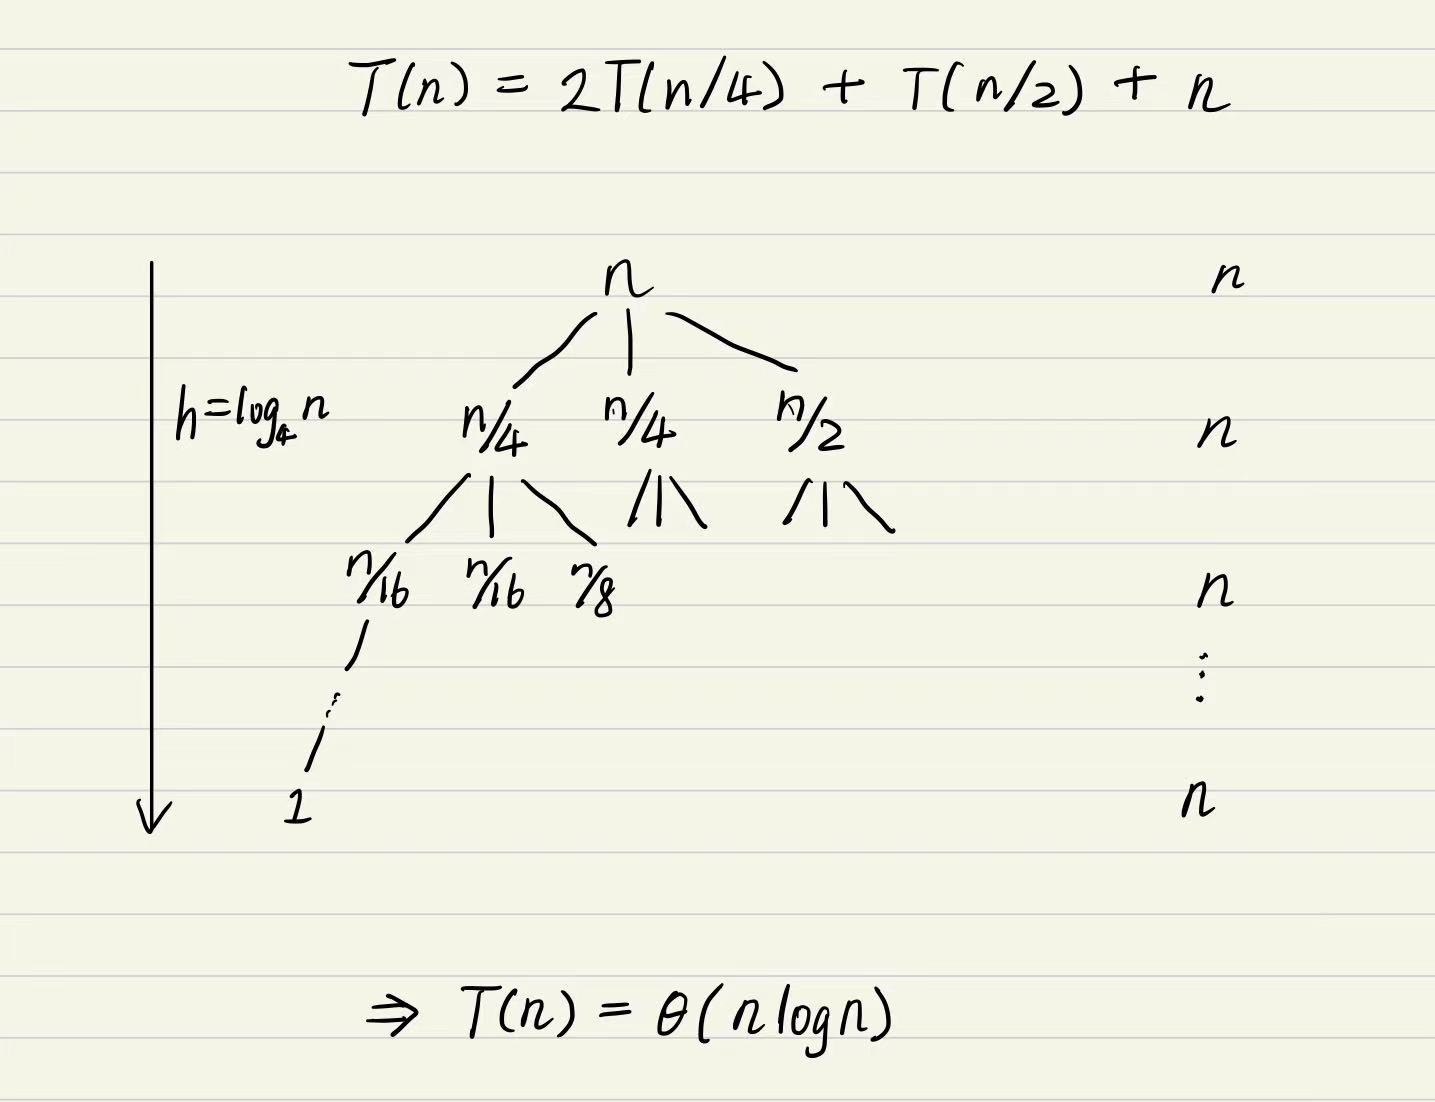
\includegraphics[width=0.5\textwidth]{1a.jpg} \\
                                \caption{The recursion tree of Problem 1a(c).}
                            \end{center}
                        \end{figure}
                  \item $T(n) = \Theta(n^{\log_45})$\\
                        Proof: $a = 5, b = 4 \Rightarrow n^{\log_ba} = n^{\log_45}; f(n) = n$. \\
                        Case 1 of Master Theorem: $f(n) = O(n^{\log_45-\eps})$ where $\eps = \log_45-1$, then $T(n) = \Theta(n^{\log_45})$.
              \end{enumerate}

        \item $T(n) = \Theta(n\log n)$\\
              Proof: \begin{figure}[H]
                  \begin{center}
                      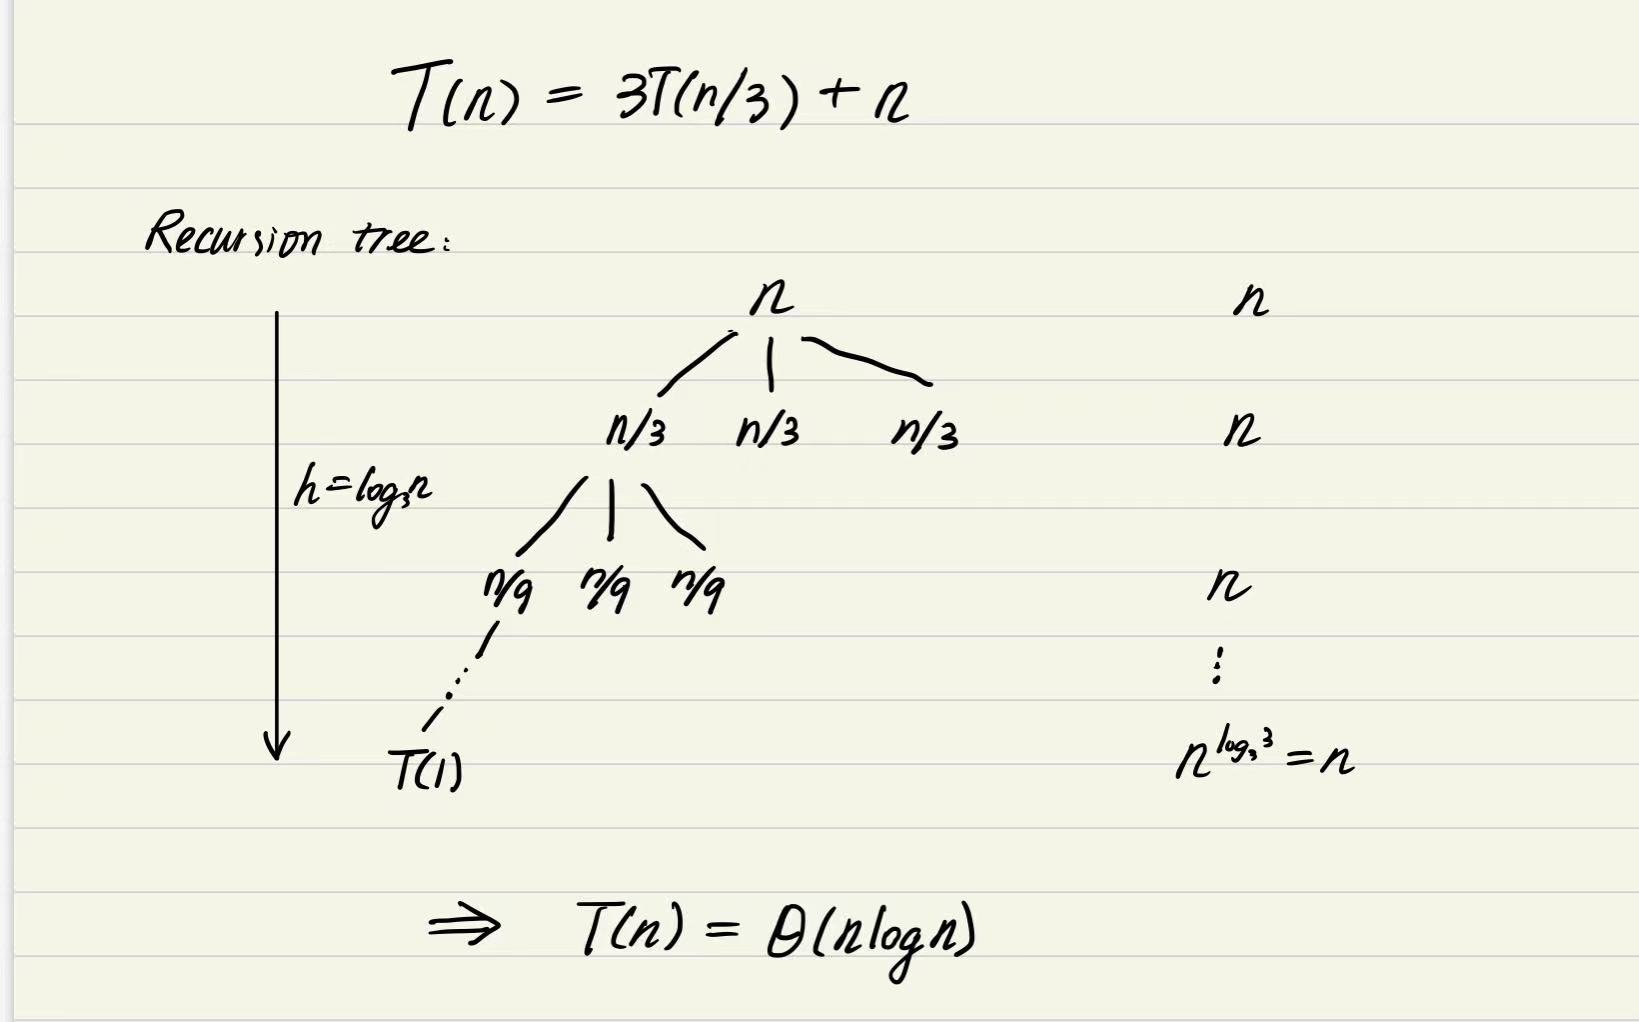
\includegraphics[width=0.5\textwidth]{1b.jpg} \\
                      \caption{The recursion tree of Problem 1b.}
                  \end{center}
              \end{figure}
    \end{enumerate}
\end{solution}

\newproblem{Rotated and Sorted}{10+10}
Suppose you are given a array of $n$ distinct numbers which was sorted and then rotated $k$ indices, for some unknown integer $k$ between 1 and $n-1$. That is, you are given an array $A[1..n]$ such that some prefix $A[1..k]$ is sorted in increasing order, the corresponding suffix $A[k+1..n]$ is also sorted in increasing order, and $A[n]<A[1]$. For example, you might be given the following 16-element array (where $k=10$): $[9, 13, 16, 20, 21, 24, 25, 26, 27, 30, ||, 1, 2, 3, 5, 6, 8]$
\begin{enumerate}[label=\alph*)]
    \item Describe and analyze an algorithm to compute the value of $k$ in $\Theta(\log n)$ time.
    \item Describe  and  analyze  an  algorithm  to  determine  if  the  given  array contains a given number $x$ that runs in $\Theta(\log n)$ time assuming you already know the value of $k$.
\end{enumerate}

\begin{solution}
    \begin{enumerate}
        \item Use binary search over the array to find $k$, as the pseudo code indicates. The time complexity is $T(n) = T(n/2) + O(1) = O(\log n)$.
              \begin{lstlisting}[language=Python]
                  start = 0, end = len(A) - 1
                  while start < end:
                    mid = (start + end) / 2
                    if A[mid] > A[end]:
                        start = mid + 1
                    else:
                        end = mid
                  return start
              \end{lstlisting}

        \item Use binary search twice over the subarrays $A[1..k]$ and $A[k+1..n]$. If the number $x$ is found in either subarray, return that the array contains $x$. Otherwise, return that the array does not contain $x$. The time complexity of this approach is $T(n) = T(k) + T(n-k) = O(\log k) + O(\log (n-k)) = O(\log n)$.
    \end{enumerate}
\end{solution}

\newproblem{Hex}{20}
Hex is a two-player game played on a diamond-shaped board made up of hexagons.  In the game, one player plays white pieces, while the other plays black, with play alternating between players and placement only allowed on unoccupied hexagons. Alternate sides of the board are designated white and black as shown above, and the goal of the game is to complete a chain of pieces between one player's two sides.

\noindent    Give an algorithm that takes as input the black pieces and white pieces on a board of length $n$ on each side, and determines whether that configuration is a winning configuration for either player. Your algorithm must employ the Union-Find data structure. See accompanying figure for an illustration.

\begin{figure}[H]
    \begin{center}
        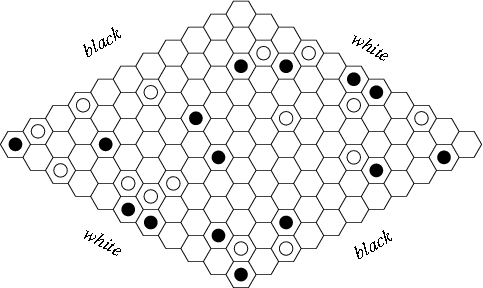
\includegraphics[width=0.7\textwidth]{files/10061--figure.png} \\
        \caption{The game is usually played on a boards of size 11 on a side, for a total of 121 hexagons. \\ \small \textcolor{gray}{Reference: \url{http://mathworld.wolfram.com/GameofHex.html}}}
    \end{center}
\end{figure}

\begin{solution}
    We can model each piece as a node and use an undirected graph represented by adjacency list to model all the pieces on the board. Each node has fields named color(black/white), isBorder(0 - inner nodes, 1 - on the left two edges of the board, 2 - on the right two edges of the board) and parent, a pointer that points to the parent node. The key is to give priority to sets containing nodes on the border when unit two sets. The pseudo code is:
    \begin{lstlisting}
        Input: Graph G(V, E)
        for node in V:
            node.parent = null
        
        for edge(node_i, node_j) in E:
            if node_i.color == node_j.color:
                parent_i, border_i = find_parent(node_i)
                parent_j, border_j = find_parent(node_j)
                if border_i + border_j == 3:
                    return true 
                unit(parent_i, parent_j)

         return false           
    \end{lstlisting}
\end{solution}

\newproblem{Thresholded Inversions and Doctor Manhattan}{20+20}

\begin{enumerate}[label=\alph*.]

    \item You'll be given an array of integers $a_i$ and a threshold value $t$ as input, describe and analyze an algorithm to determine the number of threshold inversions in the array. An inversion between indices $i < j$ is a threshold inversion if $a_i > t * a_j$, where $t$ is the threshold value given as input.

          \emph{Hint: Understanding counting inversions (normal inversions, without a threshold) will be useful to figure out how to do threshold inversions. We will be covering that in the recitations.}


    \item \textbf{Description}: Assist Doctor Manhattan in his attempt to preemptively save the world.

          \textbf{Problem Statement}: Doctor Manhattan does not see time as we know it. Due to his perception of time, he sees his past, present and future simultaneously. He has recorded tachyon levels in the present and near future. A drastic change in tachyon levels at two points in time is a critical event that should be brought to his attention since it may be cause for immense concern. It is your job to help Doctor Manhattan find these critical events. Given an array of tachyon levels in distinct points of time, compute the number of critical events.

          You are given an array $a$ which denotes tachyon levels for different points of time and a threshold factor $t$.
          For two tachyon levels, it is considered a critical event if for some $i < j$ we have $a[i] > t * a[j]$.
          You have to count the total number of such critical events.
          \textbf{Input Format}:
          First Line contains a single number which represent the threshold level. i.e. $t$

          Second Line contains the size of the array i.e. $n$

          Third line contains n elements separated by space i.e. $a[1] \ a[2] \ldots \ a[n]$

          \textbf{Constraints}:
          $0 < n < 10^5$

          $0 < a[i] < 10^9$

          $1 < t < 500$

          \textbf{Output Format}:
          Just a single number i.e. total count of critical events

          Print the answer modulo: $10^9 + 7$.

\end{enumerate}

\begin{solution}
    HackerRank username: \textbf{zhang\_lei1}
\end{solution}

\end{document}